Tässä kappaleessa käsitellään useamman vuoden käytössä ollutta ratkaisua juomien kaatamiseen Drinkkirobotilla. Ratkaisussa juomien kaadolle robottikoodissa on yksittäinen job, joka on esitetty alla.

\begin{center}
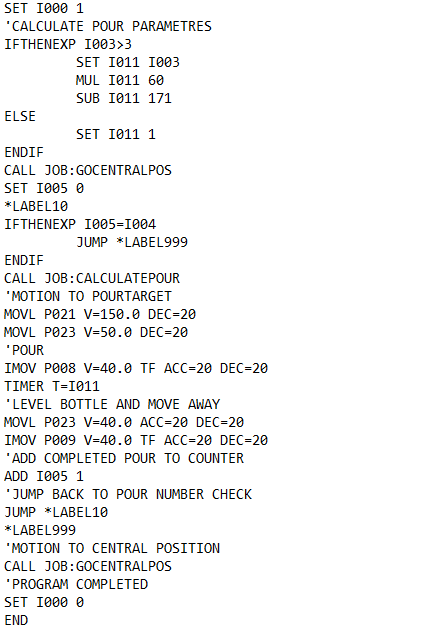
\includegraphics[scale=0.8]{img/POURDRINKS.png}
\end{center}

Kaadon tarkkuutta tarkastellessa merkittävä osa jobissa on ensimmäinen if-else-haara, joka käsittelee kaadossa käytetylle ajastimelle annetun arvon laskentaa.

Haluttu kaadon määrä senttilitroina on asetettu muuttujaan I003. POURDRINKS jobi laskee alussa ajan, jonka mukaan robotti kaataa juomaa. Kuten kuvasta nähdään, kaadon aika sekunteina saadaan kaavalla
\[t = 60 \cdot V - 171, \]
jossa V on muuttuja I003, eli haluttu tilavuus senttilitroina. Kyseessä on lineaarinen yhtälö, jossa kulmakerroin 60 ja vakiotermi -171 ovat määritetty kokeellisesti kaatamalla eri määriä juomia.

Jobi toimii siis pääpiirteittäin siten, että robotti liikkuu kohteena olevan mukin kohdalle ja kallistaa pulloa. Kun pullo on kallistunut kaatoasentoon, käynnistyy ajastin, jonka kesto on määritelty muuttujaan I011.

Ensimmäisen if-elsen tehtävä on myös tarkastaa onko haluttu kaatomäärä alle kolme senttilitraa. Tätä pienemmillä määrillä yllä kuvattu lineaarinen funktio antaisi negatiivisen ajan. Niinpä kaikilla määrillä, jotka ovat alle kolme senttilitraa, kaatoajaksi on määritelty yksi sekunti.

Kaatojobi hoitaa kaadon useammalle mukille samalla, sillä siinä käytetään silmukkaa LABEL10- ja LABEL999-lippujen sekä muuttujien I004 ja I005 avulla. Muuttuja I005 on lasin numero, johon robotti sen hetkisellä iteraatiolla kaataa. Muuttuja I004 taas on haluttujen lasillisten määrä. Jobi CALCULATEPOUR laskee koordinaatit, joissa kohdemuki on ja tallettaa sen P-alkuisiin paikkamuuttujiin. Tässä se käyttää apuna muuttujaa I005. Mukipaikat ovat vaakasuorassa rivissä, joten siirtyessä mukilta toiseen riittää vain lisätä robotin koordinaatiston x-koordinaattia mukien etäisyyden verran.
